\chapter{Premier chapitre}
\section{exemples de base}

\subsection{listes}

\begin{enumerate}
  \item {\bf Premier point (gras) ;}
  \item {\em Second point (italique) ;}
  \item {\Large Troisième point (gros) ;}
      \begin{enumerate}
          \item {\small Premier sous-point en petit}
          \item {\tiny Second sous-point (petit)}
          \item {\Huge Troisième sous-point (très gros)}
      \end{enumerate}
      
  \item[$\bullet$] {\sf Point avec une puce (sans serif)}
  \item[$\circ$] {\sc Point avec un autre style de puce (petites lettres capitales)}
\end{enumerate}


\section{exemple d'insertion d'image}
Lorem ipsum dolor sit amet, consectetur adipisicing elit, sed do eiusmod tempor incididunt ut
labore et dolore magna aliqua. Ut enim ad minim veniam, quis nostrud exercitation ullamco
laboris nisi ut aliquip ex ea commodo consequat. Duis aute irure dolor in reprehenderit in
voluptate velit esse cillum dolore eu fugiat nulla pariatur. 
\begin{figure}[h]
    \centering
    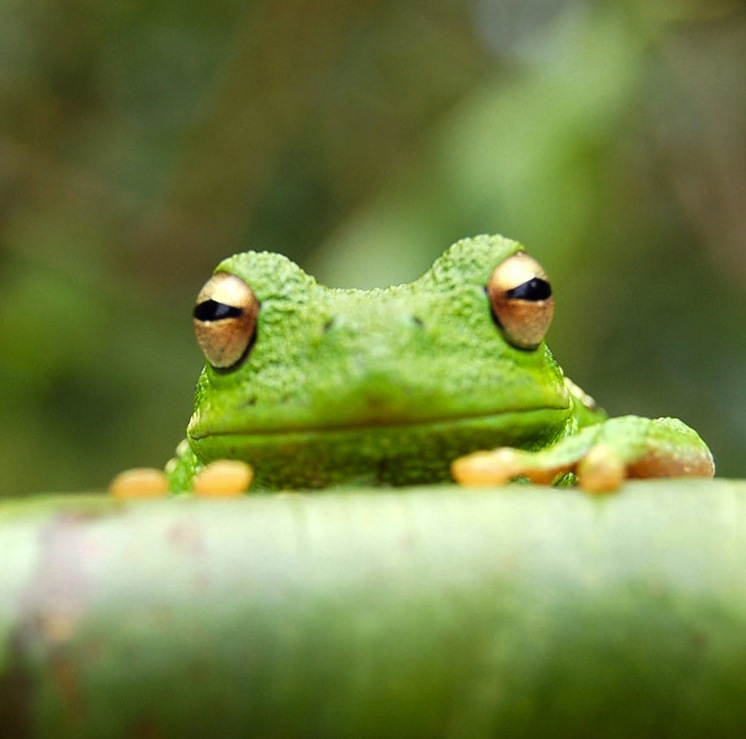
\includegraphics[width=0.2\textwidth]{images/frog.jpg}
    \caption{Illustration d'une grenouille}
    \label{fig:frog1}
\end{figure}

Excepteur sint occaecat cupidatat
non proident, sunt in culpa\ref{fig:frog1} qui officia deserunt mollit anim id est laborum.
Lorem ipsum dolor sit amet, consectetur adipisicing elit, sed do eiusmod tempor incididunt ut
labore et dolore magna aliqua. 

\section{exemple d'insertion d'un tableau}
Lorem ipsum dolor sit amet, consectetur adipisicing elit, sed do eiusmod tempor incididunt ut
labore et dolore magna aliqua. Ut enim ad minim veniam, quis nostrud exercitation ullamco
laboris nisi ut aliquip ex ea commodo consequat. Duis aute irure dolor in reprehenderit in
voluptate velit esse cillum dolore eu fugiat nulla pariatur (ex. Tableau \ref{table:1}). 
\begin{table}[h!]
    \centering
    \begin{tabular}{||c c c c||} 
     \hline
     Col1 & Col2 & Col2 & Col3 \\ [0.5ex] 
     \hline\hline
     1 & 6 & 87837 & 787 \\ 
     2 & 7 & 78 & 5415 \\
     3 & 545 & 778 & 7507 \\
     4 & 545 & 18744 & 7560 \\
     5 & 88 & 788 & 6344 \\ [1ex] 
     \hline
    \end{tabular}
    \caption{Exemple de tableau et de libellé}
    \label{table:1}
\end{table}


Excepteur sint occaecat cupidatat
non proident, sunt in culpa\ref{fig:frog1} qui officia deserunt mollit anim id est laborum.
Lorem ipsum dolor sit amet, consectetur adipisicing elit, sed do eiusmod tempor incididunt ut
labore et dolore magna aliqua. 


\section{Exemple de référence aux acronymes}
Lorem ipsum dolor \ac{MPC} sit amet, consectetur adipisicing elit, sed do eiusmod tempor incididunt ut
labore et dolore magna aliqua. Ut enim ad minim veniam, quis nostrud exercitation ullamco
laboris nisi ut aliquip ex ea commodo consequat. Duis aute irure dolor in reprehenderit in
voluptate velit esse cillum dolore eu fugiat nulla pariatur (ex. Tableau \ref{table:1}). 
